
%***************%
\chapter{Requirement Engineering and Operationalization}\label{chp:operationalization}
%***************%

%***************%
\section{Introduction}
%***************%

\begin{figure}[ht]
    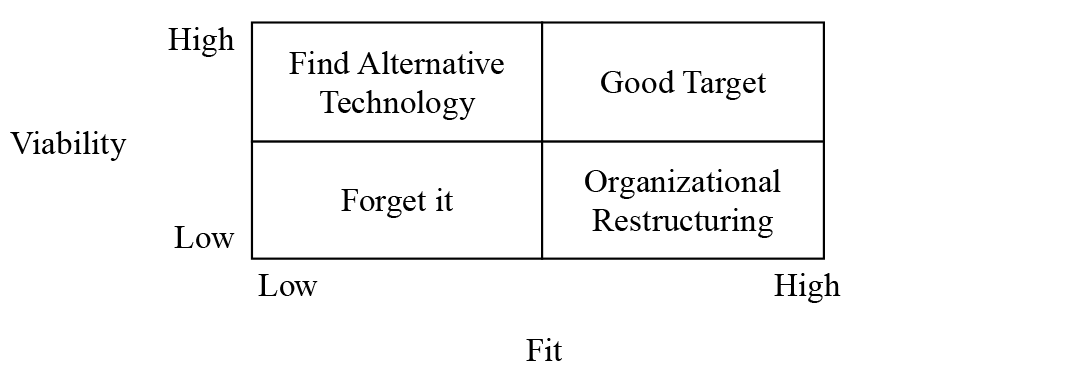
\includegraphics[width=\linewidth]{images/methodology/viabFit.PNG}\centering
    \caption
    [Viability-Fit Matrix]
    {Viability-Fit Matrix \cite{Liang2004IntroductionApplications}}
\end{figure}

In the following section, concepts and indices for measuring suitability and viability will be introduced. The insights presented in chapter \ref{chp:background} will be the foundation for the requirements and operators since the current academic and professional understanding of the topic will be assumed as correct and holistic. The steps from section \ref{sssec:reqEng} will be shortened for the upcoming sections on suitability and viability, since \textit{System Modeling} will be done in chapter \ref{chp:prototyping} and validation is discussed in chapter \ref{chp:suitabilityAssessment} and \ref{chp:viabilityAssessment} respectively.  

%***************%
\section{Suitability}
%***************%

The author defines \textit{suitability} as the measure of how well the prototype fits the environments demands and tasks characteristics. Quantifiably measurable aspects will be compared directly while disclosing the desirable value. Qualitatively measurable aspects will be discussed and deductively compared in order to study the prototypes' differences. 

\begin{figure}[ht]
    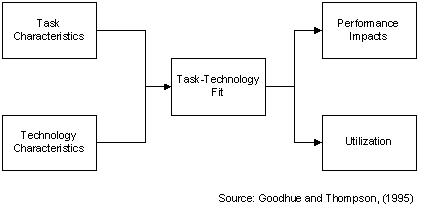
\includegraphics[width=0.7\linewidth]{images/methodology/ttf.jpg}\centering
    \caption
    [Task-Technology-Fit Model]
    {Task-Technology-Fit Model \cite{Goodhue1995Task-TechnologyPerformance}}
\end{figure}

\subsection{Identification of Requirements / Task Characteristics}

As discussed in chapter \ref{chp:background}, IoT Event-Stream-Processing entails a distinctive set of task and environment characteristics. It is characterized by an enormously high amount of client nodes that send data in a timely ordered fashion. These messages have to be processed in near real-time to avoid a system wide congestion that would result in a degradation of service and possible loss of messages. The API Gateway's performance is mostly neglectable in a real-world scenario since the computational heavy-lifting is done by the data-consumer, this characteristic results in a requirement for a processing architecture that can seamlessly handle the computational load that is resulting from any data ingress.\\
Since it is often not possible to estimate the exact amount of messages and therefore the exact amount of required compute power, the data-consumer's capacity has to \textit{automatically scale} with the load. The data ingress level can vary in short periods of, hence a manual scaling is not desirable.

Consequently, the architecture must be \textit{inherently event-driven}. If not, a fully automated scaling strategy is not possible by definition. Moreover, an event-driven approach results in an architecture that is better equipped to respond to elastic workloads, such as the ones found in IoT environments. As previously discussed, it is necessary to immediately process incoming information in an IoT context to derive valuable insights. An event-driven system is therefore well suited for this task because it \textit{minimizes the latency} between the moment of receiving the message and processing it because the information flow is strictly left-to-right. Other alternatives would introduce a lag-time by requiring the processing part of the architecture to query the data storage for new data. 

Equally important is the system's ability to "self-heal", meaning the capability to mitigate components collapse and to to maintain an operational state. This resulting \textit{failure resilience} of data-consumers is vital for an efficient Event-Stream-Processing architecture because a lack thereof will result in massive backpressure on the downstream services and API Gateway and leads to an inevitable system-wide congestion.\\
Tightly related is the tasks demand for a \textit{high throughput}. It can directly derived from the overarching need to avoid a message congestion at any cost. Naturally, a higher throughput is desirable and will lead to an increased performance and overall better suited system for the task.

Lastly, it is a characteristic of IoT Event-Processing-Tasks in a real-world business context, that cost are often calculated in a very granular fashion. Since the IoT system's monetary value is often contingent on the amount of messages processed, it is, from a business perspective, very desirable to have a system which generates costs that are directly correlated to the amount of messages processed, too. Hence, a \textit{dynamic billing based on computation} is a requirement that is not pivotal, but should be considered nonetheless.

\subsection{Specification of Requirements}

The identified requirements are therefore as follows:

\begin{enumerate}
    \item \textbf{Automated/Limitless Scaling}\\
        (Qualitatively measured)
    \item \textbf{Event-Driven Design}\\
        (Qualitatively measured) 
    \item \textbf{Low Latency}\\
        (Quantifiably measured) Message Received - Message Processed
    \item \textbf{Failure Resilience}\\
        (Qualitatively measured) Automatic Failover Strategies, Outage Mitigation, Self-Healing Capabilities
    \item \textbf{Message Throughput}\\
        (Quantifiably measured) 
\end{enumerate}



%***************%
\section{Viability}
%***************%

\textit{Viability} measures the extent of value-added by the technology in comparison to the cost of operation, development, implementation and so forth. Quantifiably measurable aspects will be compared directly while disclosing the desirable value. Qualitatively measurable aspects will be discussed and deductively compared in order to study the prototypes' differences. 

viability  measures the extent to which the environment or organization is ready fo r the application



\begin{figure}[ht]
    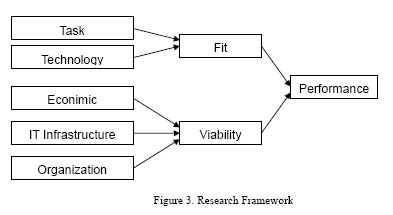
\includegraphics[width=0.7\linewidth]{images/methodology/fvm.jpg}\centering
    \caption
    [Fit-Viability-Model]
    {Fit-Viability-Model \cite{Liang2007AdoptionModel}}
\end{figure}


\subsection{Identification of Requirements / Task Characteristics}

As discussed in chapter \ref{chp:background},

\subsection{Specification of Requirements}

\begin{enumerate}
    \item \textbf{Ease of Development}\\
        (Qualitatively measured) Including: Quality/Comprehensiveness of Documentation, Available Tooling, Ease of Testing (Unit, Integration, User Acceptance, etc.), Debugging, ...
    \item \textbf{Ease of Operation}\\
        (Qualitatively measured) Including: Monitoring, Deployment, Versioning, Performance Optimization, ...
    \item \textbf{Feature Velocity}\\
        (Qualitatively measured) 
    \item \textbf{Low Vendor Lock-In}\\
        (Qualitatively measured) 
    \item \textbf{Cost}\\
        (Quantifiably measured) Including: Overall Cost of Operation/Ownership, Cost-Control, Ease of Billing/Payment, Total Costs of Maintenance, ...
\end{enumerate}


\section{Requirements Validation}\label{sec:reqVal}

In order to select a set of important system's properties for the prototype evaluation, a quantitative survey was conducted employing a Likert scale. Ten Likert items were derived from the suitability and viability requirement identification in the previous steps. The Likert items are as follows:

\begin{enumerate}[nolistsep]
    \item \textbf{Ease of Development}\\
        Including: Quality/Comprehensiveness of Documentation, Available Tooling, Ease of Testing (Unit, Integration, User Acceptance, etc.), Debugging, ...
    \item \textbf{Ease of Operation}\\
        Including: Monitoring, Deployment, Versioning, Performance Optimization, ...
    \item \textbf{Feature Velocity}
    \item \textbf{Low Vendor Lock-In}
    \item \textbf{Cost}\\
        Including: Overall Cost of Operation/Ownership, Cost-Control, Ease of Billing/Payment, Total Costs of Maintenance, ...
    \item \textbf{Automated/Limitless Scaling}
    \item \textbf{Event-Driven Design}
    \item \textbf{Low Latency}\\
         Message Received - Message Processed
    \item \textbf{Failure Resilience}\\
         Automatic Failover Strategies, Outage Mitigation, Self-Healing Capabilities
    \item \textbf{Message Throughput}
\end{enumerate}

As bipolar response categories the set \textit{Not Important} and \textit{Very Import} were chosen. In order to prevent respondents from so called "fence-sitting" (choosing the most neutral response option), an even number of scale points was used. To improve the reliability furthermore, the forced-choice response set was extended to six feedback options since a low scale score variability is expected.\autocite{Brill2008LikertScale} Similarly, a set of consecutive integers (i.e., 1, 2, 3, 4, 5, 6) was used to label the response scale to emphasize the equidistance between the options. Consequently, this setup results in an ordinal level of measurement, which can be processed by parametric statistics to gain insights on how to construct the test cases. \\
The evaluation of this survey's results will lead to one distinct system characteristic each for \textit{suitability} and \textit{viability}. For each domain, the system property with the highest measured importance among the respondents will be chosen due to the limited time and scope of this research. \\
Likert scales are subject to several academic inaccuracies and response distortion. To begin with, central tendency (respondents tend to choose the most neutral and therefore most central response option\autocite{Schumacker2013CentralDispersion}) can occur due to the interviewees impulse to avoid extreme response categories. In addition, acquiescence bias can distort the results. It refers to the tendency of respondents to choose to agree with statements because of the intention to choose what they think is the appropriate or objectively "correct" answer.\autocite{Costello2015AcquiescenceEducation}\highcomma\autocite{Aichholzer2015ControllingTests} Similarly, social desirability bias may occur when respondents try to portray themselves in a specific way.\autocite{Grimm2010SocialBias} \\
Since this survey does not address personal, moral or ethical topics, the biases mentioned above will not have a drastic influence on the results. Their impact is therefore neglectable. 


%***************%
\subsection{Results}
%***************%




%***************%
\section{Summary}
%***************%